
\titleformat{\chapter}[hang] 
{\normalfont\huge\bfseries}{\chaptertitlename\ \thechapter:}{1em}{} 

\chapter{Usability exercise}
\label{sec:usability-exercise}

\Cref{sec:usability-exercise-text}, including headings, is the exact text
of the instructions provided to volunteers so they could help asses the usability of \MultiChor.
\Cref{fig:usability-exercise-diagram} is a sequence diagram that was included with the instructions.
The volunteers, fellow graduate students with relevant experience and prior introduction to the concepts used in \MultiChor,
were not able to complete this exercise in the scheduled two-hour sessions.
These sessions were open-book/open-universe,
and included unstructured interactive guidance from the author.


\section{\MultiChor Demo Exercise}
\label{sec:usability-exercise-text}

\subsection{Instructions}

Pull the \href{https://github.com/ShapeOfMatter/MultiChor/tree/auction-demo}{MultiChor repository}:

\begin{minted}{bash}
git clone -b auction-demo git@github.com:ShapeOfMatter/MultiChor.git
\end{minted}

Enter its dir and check that you're at the HEAD of the \inlinecode[bash]{auction-demo} branch.

Run the (reduced) unit tests to confirm you're set up.

\begin{minted}{bash}
cabal test -f test
\end{minted}

This will also build the whole project, so it may take a little while the first time.
One more likely source of problems is your GHC version;
version 9.10.1 is preferred.

Open \inlinecode[bash]{examples/Auction.hs}.
Observe that there's an example choreography \inlinecode[bash]{auction} on line~33.
You'll be editing this to correctly implement the below protocol.

The goal here is to find specific short-comings of MultiChor as a library that people might actually use.
The goal is \emph{not} to test your own skill, or acquire a perfect implementation of the below protocol.
Set yourself a timer for two hours, and quit when it goes off.
Ask Mako questions, including about how to do particular things, at any point.


\subsection{Exercise}

A group of companies are setting up an automated system
that will run at midnight every night to set the price of doodads for the following day.
Five of the companies are buyers, and there is one seller.
There is also a "proctor" participant, who provides some oversight.
This will be a semi-blind Vickrey auction:
Each of the buyers will send their bids to the seller,
who will inform everyone of the bid amount and identities of the top two bids.
Because the parties are all well-informed and doodads don't change much in value from one day to the next,
ties are likely.
In the event of a tie, preference will be given to the various parties randomly.
The parties trust each other; multi-round commitments are considered unnecessary.

Here is the specific protocol:
\begin{enumerate}
  \item All buyers send their bids to the seller and the proctor.
  \item \textbf{IF AND ONLY IF} there is a (possibly many-way) tie for highest bid:  
    \begin{itemize}
      \item The proctor randomly chooses one of the highest-bidding buyers and sends that choice to the seller.
    \end{itemize}
  \item The seller sends everyone the two tuples (winner, bid) and (second-place, bid).
   In the case of a many-way tie, it doesn't matter who is chosen as second-place.
 \item All parties print the name of the winner and the amount of the second-place bid.
\end{enumerate}

\subsection{\textit{Nota bene}}
\begin{itemize}
  \item \href{https://hackage.haskell.org/package/MultiChor}{The Hackage documentation} may be easier to navigate than the source code in \inlinecode{src/},
  but it may be a little out of date.
  In particular, we used to use the word "enclave" instead of "conclave".
  \item If you need a \inlinecode[bash]{KnownSymbol} or \inlinecode[bash]{KnownSymbols} constraint, you can usually just add it wherever you need it.
  \item If you need to work with a \inlinecode[bash]{Quire}, notice that its instances for \inlinecode[bash]{Functor} \textit{etc} don't give you access to the party names;
    you can use \inlinecode[bash]{stackLeaves} to make a new \inlinecode[bash]{Quire} and \inlinecode[bash]{toLocTm} to get the term-level name of a party.
  \item The monad \inlinecode[bash]{CLI IO} is a shim around \inlinecode[bash]{IO}.
    It satisfies \inlinecode[bash]{MonadIO} (so you can always use \inlinecode[bash]{liftIO}),
    and it affords \inlinecode[bash]{getInput} and \inlinecode[bash]{putOutput},  which are like normal input and output except they can be mocked during testing.
  \item Most of the test cases have been de-activated so you can run the tests quickly and often.
    Should you want to turn them all back on, change \inlinecode[bash]{examples/Tests.hs} line~41.
  \item Effectively calling `main` via `cabal run...` would require coordinating seven open shells; I don't suggest you bother.
\end{itemize}

\begin{figure}[tbhp]
  \begin{mdframed}
  \begin{tabular}{c}
  \begin{minipage}{13.5cm}
    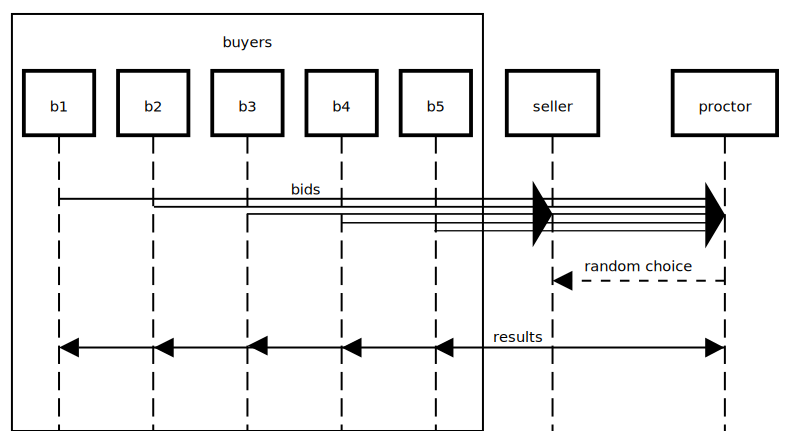
\includegraphics[width=13.5cm]{exercise.pdf}
  \end{minipage}
  \end{tabular}
  \caption{sequence diagram}
  \label{fig:usability-exercise-diagram}
    %%\Description{In the top section, twenty four lines of Haskell code using the MultiChor library, with a UML sequence diagram of that program.
%%	  }
  \end{mdframed}
\end{figure}
